\documentclass[12pt]{article}

% Packages
\usepackage{sbc-template}
\usepackage{graphicx,url}
\usepackage[brazil]{babel}   
\usepackage[utf8]{inputenc}  
\usepackage{lipsum}

\sloppy

% Info
\title{On extracting reaction semantics from high level languages}
\author{Alek Frohlich\inst{1}, Gustavo Biage\inst{1}}
\address{Departamento de Informatica e Estatística – Universidade Federal de Santa Catarina \\
Florianopolis – SC – Brazil
  \email{\{alek.frohlich,gustavo.c.biage\}@grad.ufsc.br}
}

\begin{document} 

\maketitle

\begin{abstract}
    The growth of research areas such as synthetic biology and systems biology leads to an increased willing to develop new, larger mathematical models to describe complex biological behavior. In order to enable natural flow of development of those models, scientists must have access to tools which increase the level of abstraction and enable reuse of biological components. Increased efforts are being put on solving these two problems.
    % fix cohesion
    Thus, the present work tackles the question of reuse by integrating the existing programming language Gro with SBML for model interchangeability.
\end{abstract}

\section{Introduction}
    \lipsum[1]

\section{Albi: a simple Gro parser}
    \lipsum[1]

\section{Study case: The Repressilator}
    \lipsum[1]

\subsection{Mathematical Model}
    \lipsum[1]
    % Cite example
    \cite{Hucka2003}
    % Figure example
    (Figure~\ref{fig:repressilator}).

% Oscillation
\begin{figure}[ht]
\centering
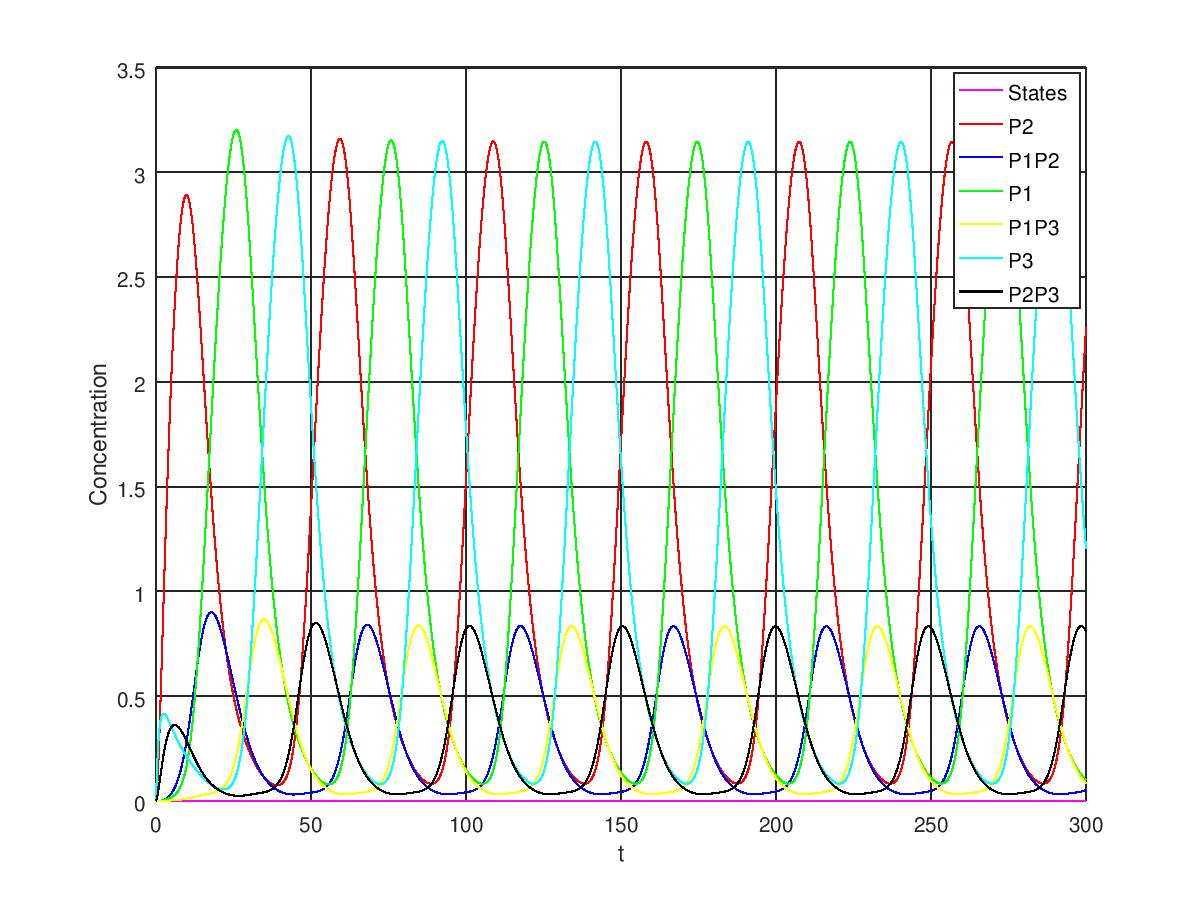
\includegraphics[width=.5\textwidth]{repressilator.jpg}
\caption{Repressilator}
\label{fig:repressilator}
\end{figure}

% EPS generated from Octave
% \begin{center}
%     \begin{figure}[h]
        
%         \begin{subfigure}
%             \includegraphics[scale = 0.4]{my_plot-inc.eps}
%             \caption{Caption1}
%             \label{fig:subim1}
%         \end{subfigure}
%         \begin{subfigure}
%             \includegraphics[scale = 0.4]{my_plot-inc.eps}
%             \caption{Caption1}
%             \label{fig:subim1}
%         \end{subfigure}
%     \end{figure}
%     % \setlength{\unitlength}{1pt}
%     % \begin{picture}(0,0)
%     % \includegraphics[scale = 0.4]{my_plot-inc}
%     % \end{picture}%
%     % \begin{picture}(576,432)(0,0)
%     % \fontsize{10}{0}
%     % \end{picture}
% \end{center}

\subsection{Extracting behavior from Gro}
    \lipsum[1]
    
\subsection{Simulating output on Copasi}
    \lipsum[1]

\section{Conclusion}
    \lipsum[1]
    
\section{Future works}
    \lipsum[1]

% References
\bibliographystyle{sbc}
\bibliography{sbc-template}

\end{document}